% S_supplement.tmpl.tex: supplementary material (SPEC s11 "08, 09, S"; REVISION_1).
% S1: deviations, audit trail and the 2016 development table (keys from paper/ALLOW_DEV_KEYS.txt only).
% S2 figures and S3 tables, including the floats moved from the main text in REVISION_1 (H1 figure, H2 forest, sensitivity
% figure, data table, secondary table, full methods table) and the per-method cost table.
% Numbering: sections, tables and figures carry the prefix S. Labels: figS:*, tabS:* (tab:bridge kept).

\setcounter{section}{0}
\renewcommand{\thesection}{S\arabic{section}}
\setcounter{table}{0}
\renewcommand{\thetable}{S\arabic{table}}
\setcounter{figure}{0}
\renewcommand{\thefigure}{S\arabic{figure}}

\section*{Supplementary material}

Section, figure, table and equation numbers without the prefix S, and all reference numbers in brackets, refer to the main text and its reference list.

\section{Deviations, audit trail and development results}\label{sec:S1}

\subsection{Deviations from the frozen plan and post-freeze register}\label{sec:S1:dev}

The analysis plan was frozen with an md5 manifest before the 2017 evaluation. The frozen deviation file records one deviation from the plan, DEV-1, below. Every other choice and analysis made after the freeze is dated in a post-freeze register (\texttt{research/DEVIATIONS\_POST.md} in the archive), with the 2017 information known at the time. The register extends the frozen file without editing it, so the manifest hash still holds.

\paragraph{DEV-1 (code only)} The first 2017 run stopped with a missing-key error before any statistic or ledger row was computed. In final mode the synthetic-control loop had computed only the frozen SCM-ridge baseline and not the frozen SCM-classic baseline that a secondary table needs. The code was changed to compute both. The change was verified on the 2016 data, where the final-mode path reproduced every development estimate and Holm-adjusted $p$-value for H1 to H5 exactly. The manifest was reissued, and the earlier version is kept. No 2017 estimate had been seen when the change was made.

\paragraph{Further disclosures} The development-year pilot of the repeated-dispatch test contained a coding error in which donors were curtailed. It was fixed before the freeze. The status line inside the plan file predates the freeze and still reads as a draft, although its content is the frozen text; the file was left unedited so that its hash holds, and the dated manifest is the record of the freeze. The pre-registered LightGBM and MLP searches ran after the confirmatory evaluation, on 2016 data only. Their spaces, budgets and seeds were pre-registered, and the tuning score was set after the freeze and before any 2017 evaluation of the tuned variants. None of these changes used a 2017 result.

\paragraph{Post-freeze register} The register has 38 entries in four groups. The first group restores definitions of the plan: the labels of the H5 per-site slopes and the H4 headline estimand. It also restores the status of the 16:00 to 20:00 window, the opposite daylight-saving mapping and the non-event and flatline-off reruns, which the plan lists as secondary and an earlier draft called exploratory. The second group holds pre-registered runs completed after the freeze: the LightGBM and MLP searches, for which only the tuning score was chosen after the freeze, and the further pre-specified analyses of Section~\ref{sec:S1:inventory}. The third group holds analyses decided after the 2017 confirmatory results were seen. These are the bridge metrics, site intervals and payment shares, the break-even in kWh, the rank correlation, the ten-day SCM-ridge window, the mirror test, the early-shaping variants and the cross-window H5 contrast. They also include the descriptive additions of this version: the event-day table, the Clopper-Pearson bounds, the prediction intervals, the tipping value and the practitioner units. The fourth group holds wording, title and status changes. No entry changed a frozen key, frozen code or a confirmatory result. Table~\ref{tabS:inventory} gives the status of every analysis.

\subsection{Audit trail}\label{sec:S1:audit}

Two audits bracket the 2017 run. Before the freeze, a gate audit compared the written plan with the logged decisions and required the plan to be corrected where the two disagreed. After the run, a second audit checked four things. The md5 manifest still matched every frozen file. An independent script, which does not import the analysis code, recomputed every confirmatory value from the saved event tables. A leakage spot check confirmed, for sampled building-events, that lookback days are weekdays that are neither holidays nor event days and that donors sit in the opposite fold. Finally, each number in the manuscript enters through a ledger key and the build fails on a missing key. The audit reports, scripts and outputs are archived with the code at [archive DOI to be inserted at acceptance]. The leakage assertions are in \texttt{src/run/leakage.py}, the unit tests in \texttt{tests/}, and the archive README gives the rerun command and the expected audit output.

The pre-specified secondary reruns are the 16:00 to 20:00 window reruns of H4 and H5, the opposite daylight-saving mapping, and the non-event and flatline-off reruns of the flat-meter filter; Sections~\ref{sec:results:h5} and~\ref{sec:results:robust} of the main text report them. The exploratory runs, decided after the 2017 results, are the early-shaping variant a, the mirror test with a pre-event decrease, the break-even expressed in kWh, SCM-ridge with a ten-day pre-period and the cross-window H5 contrast; Section~\ref{sec:results:explore} reports them. All of these stay outside the Holm family, and their p-values are unadjusted.

\subsection{Analysis inventory and further pre-specified analyses}\label{sec:S1:inventory}

Table~\ref{tabS:inventory}, at the end of this supplement, lists every analysis unit with its status, where it is reported and its ledger keys. The following analyses have no other text report. All but the last are pre-specified, and all are outside the Holm family.

\paragraph{R2-LOO event rule} With the ten weekdays of highest site load, excluding the target, as events, the relMAE was {{method.pjmA.R2LOO.relMAE_median|pct1}} for PJM-adj, {{method.cgA.R2LOO.relMAE_median|pct1}} for CG-adj and {{method.pjm0.R2LOO.relMAE_median|pct1}} for unadjusted PJM (keys \texttt{method.<m>.R2LOO.*}). The plan lists this rule among the secondary sensitivities, and its event-rule table labels it exploratory because it selects days on donor outcomes; the ledger holds no SCM-ridge value for it.

\paragraph{Heterogeneous increase} With building increases drawn from $U(0,2p)$ at $p=0.05$, the pooled relMAE of PJM-adj was {{hetp.p0.05.pjmA.relMAE_median|pct1}}, against {{precool.relMAE.pjmA.4h.p0.05|pct1}} for the uniform increase, and SCM-ridge stayed at {{hetp.p0.05.scmR.relMAE_median|pct1}} (keys \texttt{hetp.*}).

\paragraph{First crossing $D_\tau$} The first $K$ at which $\rho$ falls 0.10 below its $K=10$ value lay beyond the tested range ($K>40$) for PJM-adj, CG-adj, CAISO-adj and SCM-ridge, and was {{H5.Dtau.pjm0|.1f}} for unadjusted PJM (keys \texttt{H5.Dtau.*}).

\paragraph{Two-point slope} The decline of the building-pooled median $\rho$ per dispatch between $K=10$ and $K=40$ was {{H5.eta_2pt.pjm0|.4f}} for unadjusted PJM, {{H5.eta_2pt.pjmA|.4f}} for PJM-adj and {{H5.eta_2pt.scmR|.4f}} for SCM-ridge, in line with the signed curves of main-text Fig.~\ref{fig:dispatch}b (keys \texttt{H5.eta\_2pt.*}).

\paragraph{Donor ablation drop-corr10} Dropping the 10\,\% of donors most correlated with the target gave a CG-adj log error ratio against the whole pool of {{ablation.donor.drop_corr10.logratio_vs_wholepool|.3f}} (interval {{ablation.donor.drop_corr10.logratio_vs_wholepool:ci_low|.3f}} to {{ablation.donor.drop_corr10.logratio_vs_wholepool:ci_high|.3f}}), a small loss of accuracy (keys \texttt{ablation.donor.drop\_corr10.*}).

\paragraph{Secondary rule family} Holm within the family of the three secondary rules (NYISO, CAISO, ISO-NE), as the plan promises, gave {{H1s.p_holm_family.ny|.5f}}, {{H1s.p_holm_family.caiso|.5f}} and {{H1s.p_holm_family.isone|.5f}} for the H1 endpoint and {{H2s.p_holm_family.ny|.5f}}, {{H2s.p_holm_family.caiso|.5f}} and {{H2s.p_holm_family.isone|.5f}} for H2. Read as one family of six, the adjusted values were {{H1s.p_holm_family6.ny|.5f}} for every rule (keys \texttt{H1s.p\_holm\_family*}, \texttt{H2s.p\_holm\_family*}).

\paragraph{Cross-window H5 contrast (exploratory)} The paired contrast of the site slope differences, 14:00 to 18:00 minus 16:00 to 20:00, was {{exploratory.h5_window_contrast.eta_diff_1418_minus_1620|.4f}} (interval {{exploratory.h5_window_contrast.eta_diff_1418_minus_1620:ci_low|.4f}} to {{exploratory.h5_window_contrast.eta_diff_1418_minus_1620:ci_high|.4f}}; unadjusted two-sided p = {{exploratory.h5_window_contrast.p_signedrank_two_sided_unadjusted|p}}). The contrast was stronger at 14:00 to 18:00 at {{exploratory.h5_window_contrast.n_sites_stronger_1418|int}} of {{sample.n_sites|int}} sites, and the Spearman correlation of the site values across windows was {{exploratory.h5_window_contrast.spearman_rho|.2f}}. The windows are not pooled, chosen between or Holm-adjusted together (keys \texttt{exploratory.h5\_window\_contrast.*}).


\subsection{Development-year results}\label{sec:S1:devtable}

Table~\ref{tabS:dev} shows the 2016 development results. They were used to fix the design before the freeze. They are labeled ``development (2016), not a result'' and are not evidence for any claim in the main text. The 2016 and 2017 verdicts for H1 and H3 differ, which Section~\ref{sec:discussion} discusses.

\begin{table}[htbp]
\centering
\caption{Development (2016), not a result: estimates and Holm-adjusted $p$-values from the development year.}\label{tabS:dev}
\footnotesize
\begin{tabular}{@{}l>{\raggedright\arraybackslash}p{6.2cm}rrr@{}}
\toprule
Hypothesis & Quantity (development (2016), not a result) & Estimate & Interval & Holm $p$ \\
\midrule
H1 & bias difference, PJM, hot minus random days & {{H1.delta_bias.pjm0_v0|.3f}} & [{{H1.delta_bias.pjm0_v0:ci_low|.3f}}, {{H1.delta_bias.pjm0_v0:ci_high|.3f}}] & {{H1.p_holm_v0:p_holm|p}} \\
H2 & log ratio of relMAE, PJM-adj over PJM & {{H2.logratio.pjmA_pjm0_v0|.3f}} & [{{H2.logratio.pjmA_pjm0_v0:ci_low|.3f}}, {{H2.logratio.pjmA_pjm0_v0:ci_high|.3f}}] & {{H2.p_holm_v0:p_holm|p}} \\
H3 & log ratio of relMAE, CG-adj over PJM-adj & {{H3.logratio.cgA_pjmA_v0|.3f}} & [{{H3.logratio.cgA_pjmA_v0:ci_low|.3f}}, {{H3.logratio.cgA_pjmA_v0:ci_high|.3f}}] & {{H3.p_holm_v0:p_holm|p}} \\
H4 & median site break-even pre-event increase, four-hour shape & {{H4.median_site_pcross_v0|.3f}} & [{{H4.median_site_pcross_v0:ci_low|.3f}}, {{H4.median_site_pcross_v0:ci_high|.3f}}] & {{H4.p_holm_v0:p_holm|p}} \\
H5 & slope difference, PJM-adj minus SCM-ridge & {{H5.eta_diff_v0|.4f}} & [{{H5.eta_diff_v0:ci_low|.4f}}, {{H5.eta_diff_v0:ci_high|.4f}}] & {{H5.p_holm_v0:p_holm|p}} \\
\bottomrule
\end{tabular}
\par\smallskip{\footnotesize\raggedright Development data, {{H1.delta_bias.pjm0_v0:n_sites|int}} sites, not frozen. H3 decision in the development year: {{H3.decision_v0}}. The H3 equivalence test had a raw $p$ of {{H3.p_tost_v0:p_raw|p}}. Intervals are the plan's bootstrap or Hodges-Lehmann intervals for the same estimands as in the main text.\par}
\end{table}

\clearpage
\section{Supplementary figures}\label{sec:S2}

Figures~\ref{figS:h1bias} to~\ref{figS:robustness} support the confirmatory tests of the main text, and Figures~\ref{figS:age} to~\ref{figS:portfolio} the stress-test diagnostics, the shaping placement, sensitivity runs and secondary portfolio analysis.

\begin{figure}[htbp]
\centering
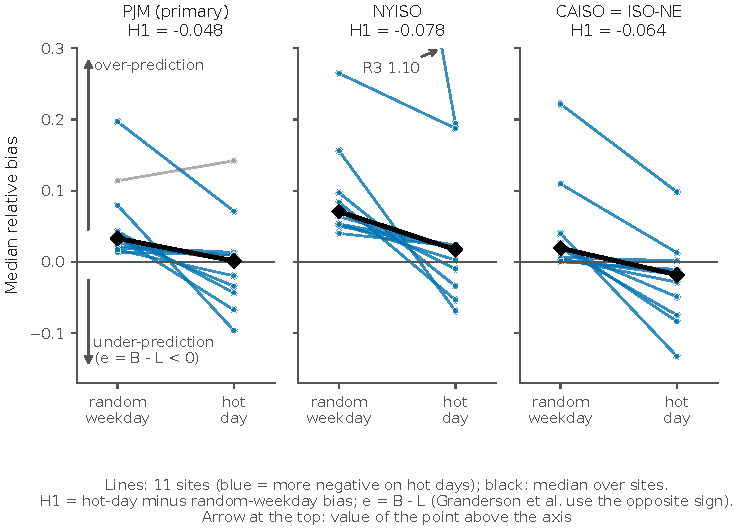
\includegraphics[width=0.8\linewidth]{figures/fig_04_h1_bias.pdf}
\caption{Replication of H1: the hot-day bias of unadjusted PJM is more negative than its random-weekday bias (difference negative at {{derived.H1.n_sites_negative|int}} of {{sample.n_sites|int}} sites). Lines connect site values. Negative means under-prediction ($e=B-L$); the sign of Granderson's NMBE is opposite.}\label{figS:h1bias}
\end{figure}

\begin{figure}[htbp]
\centering
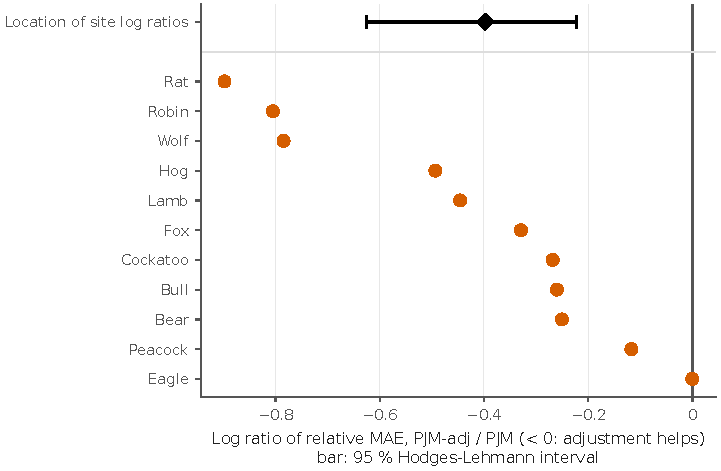
\includegraphics[width=0.78\linewidth]{figures/fig_15_h2_forest.pdf}
\caption{H2 replication: site-level log ratios of relMAE, PJM-adj over PJM ({{sample.n_sites|int}} sites), negative at {{derived.H2.n_sites_negative|int}} sites, with the Hodges-Lehmann estimate and its 95\,\% interval.}\label{figS:h2}
\end{figure}

\begin{figure}[htbp]
\centering
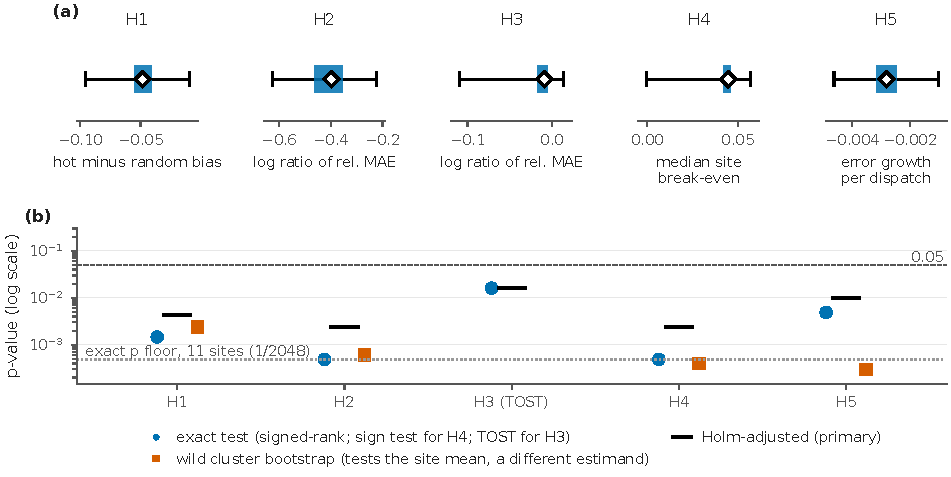
\includegraphics[width=\linewidth]{figures/fig_11_robustness.pdf}
\caption{Sensitivity analyses of the five confirmatory tests at {{sample.n_sites|int}} sites: leave-one-site-out ranges (an influence analysis) and wild cluster bootstrap $p$-values beside the exact $p$-values. The bootstrap targets the site mean, a different estimand from the site-level estimands of the primary tests. The line marks the exact $p$ floor for {{sample.n_sites|int}} sites.}\label{figS:robustness}
\end{figure}

\begin{figure}[htbp]
\centering
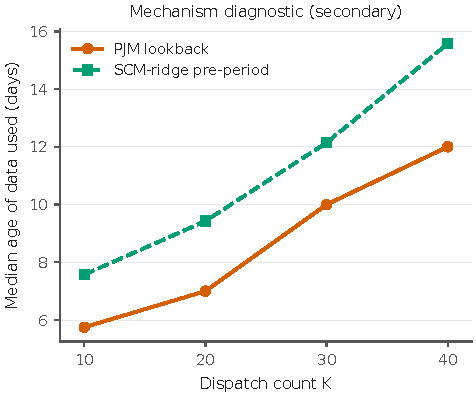
\includegraphics[width=0.56\linewidth]{figures/fig_09_age.pdf}
\caption{Age of the information that each method reads under repeated dispatch (stress test). The median age of the PJM lookback days grows from {{H5.age_days.pjm_lookback.K10|.1f}} days at $K=10$ to {{H5.age_days.pjm_lookback.K40|.1f}} days at $K=40$, and that of the SCM-ridge pre-period from {{H5.age_days.scmR_preperiod.K10|.1f}} to {{H5.age_days.scmR_preperiod.K40|.1f}} days.}\label{figS:age}
\end{figure}

\begin{figure}[htbp]
\centering
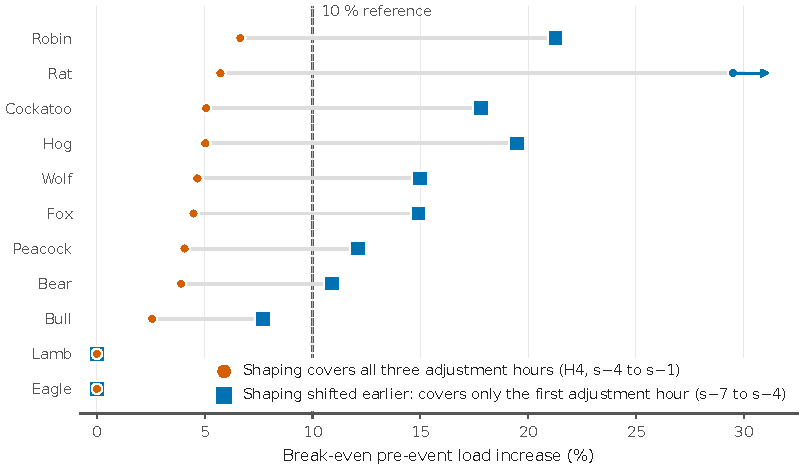
\includegraphics[width=0.875\linewidth]{figures/figS_placement.pdf}
\caption{Injected stress test: where the shaping is placed relative to the adjustment hours. Break-even pre-event load increase of PJM-adj against SCM-ridge at each of {{sample.n_sites|int}} sites, for two placements. Circles: the four-hour shaping covers all three adjustment hours ($s-4$ to $s-2$; H4, hours $s-4$ to $s-1$; median {{H4.median_site_pcross|pct1}}). Squares: it is shifted earlier so that it overlaps only the first of the three adjustment hours (early shape a, hours $s-7$ to $s-4$; exploratory; median {{exploratory.early_shape.a.pcross_samep.median_site|pct1}}). The squares compare the two methods at the same increase; the main text quotes the median against SCM-ridge without an increase, the H4 definition ({{exploratory.early_shape.a.pcross_frozenstyle.median_site|pct1}}). The dashed line is the 10\,\% reference. The break-even is below 10\,\% at {{derived.H4.n_sites_pcross_lt_threshold|int}} of {{sample.n_sites|int}} sites for the overlapping placement and at {{exploratory.early_shape.a.pcross_samep.sign_k_below_0.10|int}} sites for the early placement. Eagle and Lamb are zero in both placements. The Rat value exceeds the grid maximum (arrow). The full-coverage placement is a worst-case bound for PJM-adj, and shaping that touches no adjustment hour leaves PJM-adj unchanged by construction.}\label{figS:placement}
\end{figure}

\begin{figure}[htbp]
\centering
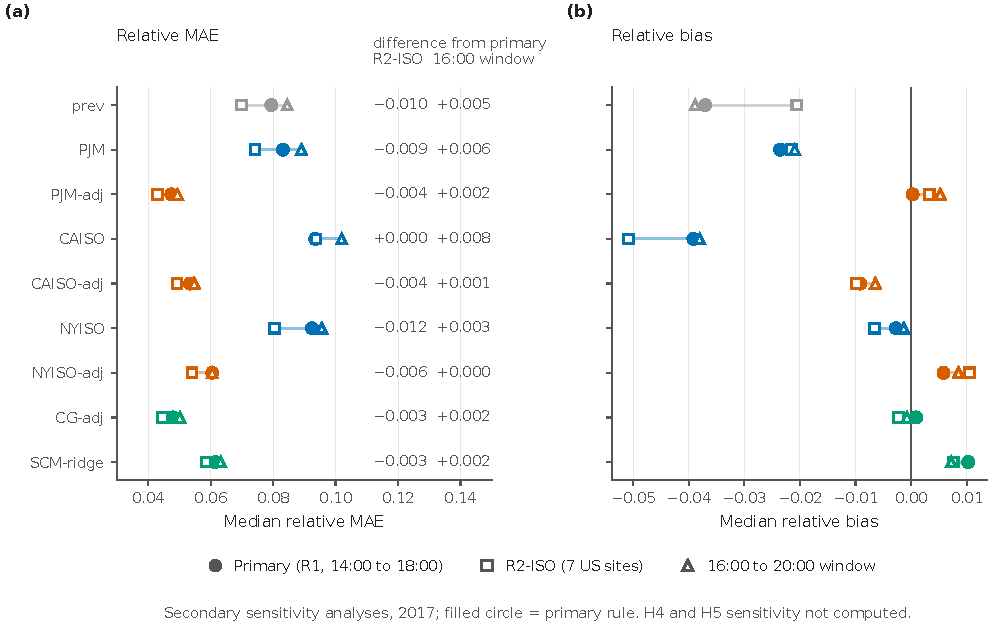
\includegraphics[width=\linewidth]{figures/fig_13_sensitivity.pdf}
\caption{Sensitivity of method accuracy and bias to the alternative event definition (R2-ISO) and to the 16:00 to 20:00 window. Only relMAE and bias are shown; no break-even pre-event increase was computed for R2-ISO, and the 16:00 to 20:00 break-even is a pre-specified secondary run (main-text Section~\ref{sec:results:robust}).}\label{figS:sensitivity}
\end{figure}

\begin{figure}[htbp]
\centering
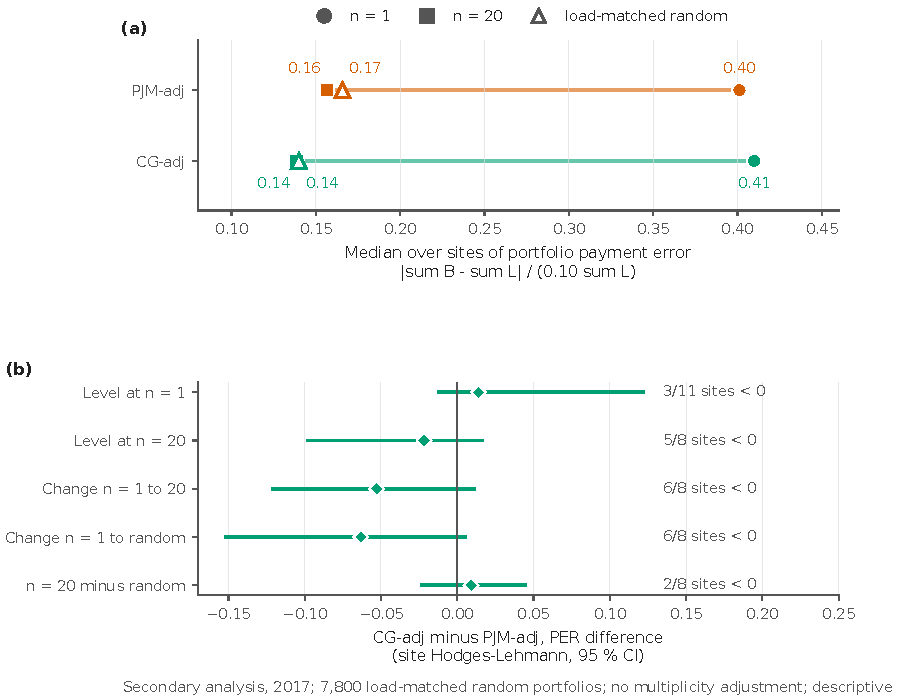
\includegraphics[width=\linewidth]{figures/fig_12_portfolio.pdf}
\caption{Pooled payment error ratio of PJM-adj and CG-adj for a single building, a 20-building portfolio and a load-matched random portfolio (secondary analysis H6). For PJM-adj the ratios are {{H6.pjmA.PER.n1|.3f}}, {{H6.pjmA.PER.nbig|.3f}} and {{H6.pjmA.PER.rand|.3f}}; for CG-adj they are {{H6.cgA.PER.n1|.3f}}, {{H6.cgA.PER.nbig|.3f}} and {{H6.cgA.PER.rand|.3f}}.}\label{figS:portfolio}
\end{figure}

\clearpage
\section{Supplementary tables}\label{sec:S3}

Tables~\ref{tabS:data} to~\ref{tabS:methodsfull} give the eligibility and event days by site, the secondary analyses, the stress-test diagnostics, the bridge to the M\&V literature, the per-method computational cost and the full list of baseline methods; Table~\ref{tabS:inventory} closes the supplement with the analysis inventory.

\begin{table}[htbp]
\centering
\caption{Data and eligibility by site (2017): timestamp convention, meters kept after each filter, whether the site enters the sample, and hot-day building-events (R1). E1 is the valid-day filter, E3 the flat-meter filter and E4 the minimum number of meters per site. Timestamp convention: STD, standard time all year; CLOCK, local clock time with a clear daylight-saving signal; AMBIGUOUS, no clear signal, mapped to clock time.}\label{tabS:data}
\footnotesize
\setlength{\tabcolsep}{3pt}
\begin{tabular}{>{\raggedright\arraybackslash}p{1.6cm}>{\raggedright\arraybackslash}p{2.3cm}>{\raggedleft\arraybackslash}p{1.4cm}>{\raggedleft\arraybackslash}p{1.9cm}>{\raggedleft\arraybackslash}p{1.7cm}>{\raggedleft\arraybackslash}p{1.5cm}>{\raggedright\arraybackslash}p{1.9cm}>{\raggedleft\arraybackslash}p{2.0cm}}
\toprule
Site & Timestamp convention & E1 meters & Flat-meter excl. (E3) & Duplicates dropped & Meters after E3 & In sample (E4) & R1 building-events \\
\midrule
Bear & CLOCK & 77 & 2 & 0 & 75 & yes & 711 \\
Bobcat & AMBIGUOUS & 9 & 0 & 0 & 9 & no (E4) & 0 \\
Bull & CLOCK & 110 & 8 & 0 & 102 & yes & 986 \\
Cockatoo & AMBIGUOUS & 90 & 0 & 0 & 90 & yes & 873 \\
Eagle & STD & 90 & 3 & 4 & 83 & yes & 663 \\
Fox & CLOCK & 128 & 1 & 0 & 127 & yes & 1{,}263 \\
Gator & AMBIGUOUS & 61 & 61 & 0 & 0 & no (E4) & 0 \\
Hog & CLOCK & 136 & 1 & 0 & 135 & yes & 1{,}301 \\
Lamb & AMBIGUOUS & 121 & 99 & 0 & 22 & yes & 87 \\
Moose & STD & 9 & 0 & 0 & 9 & no (E4) & 0 \\
Peacock & CLOCK & 36 & 0 & 0 & 36 & yes & 357 \\
Rat & STD & 255 & 2 & 0 & 253 & yes & 2{,}502 \\
Robin & AMBIGUOUS & 51 & 4 & 0 & 47 & yes & 465 \\
Wolf & STD & 35 & 0 & 0 & 35 & yes & 342 \\
All sites &  & 1{,}208 & 181 & 4 & 1{,}023 & 11 of 14 & 9{,}550 \\
\bottomrule
\end{tabular}

\end{table}

\begin{table}[htbp]
\centering
\caption{Event days and heat episodes by site, 2017. Scored days are hot-day (R1) days with at least one scored building-event ({{sample.event_days.total|int}} in all); designated days are those listed in the frozen event-date file. Lamb has {{sample.event_days.Lamb|int}} scored event days of {{sample.event_days_designated.Lamb|int}} designated, in {{sample.heat_episodes.Lamb|int}} heat episodes. A heat episode is a run of event days at most three calendar days apart.}\label{tabS:events}
\small
\setlength{\tabcolsep}{4pt}
\begin{tabular}{lrrrr}
\toprule
Site & Scored event days & Designated days & Heat episodes (scored) & Heat episodes (designated) \\
\midrule
Bear & 10 & 10 & 6 & 6 \\
Bull & 10 & 10 & 5 & 5 \\
Cockatoo & 10 & 10 & 6 & 6 \\
Eagle & 10 & 10 & 5 & 5 \\
Fox & 10 & 10 & 3 & 3 \\
Hog & 10 & 10 & 8 & 8 \\
Lamb\textsuperscript{a} & 4 & 10 & 2 & 5 \\
Peacock & 10 & 10 & 5 & 5 \\
Rat & 10 & 10 & 4 & 4 \\
Robin & 10 & 10 & 4 & 4 \\
Wolf & 10 & 10 & 6 & 6 \\
All sites & 104 & 110 & 54 & 57 \\
\bottomrule
\end{tabular}
\par\smallskip{\footnotesize\raggedright Scored event days are the hot-day (R1) days with at least one scored building-event; designated days are the 10 R1 days per site listed in the frozen event-date file. A heat episode is a run of event days at most 3 calendar days apart, so a new episode starts when the gap to the previous event day exceeds 3 days. \textsuperscript{a}Lamb has 4 scored event days (2017-07-05, 2017-07-06, 2017-07-17, 2017-07-18; 21 to 22 buildings each) in 2 heat episodes, although 10 days were designated; the other designated days carry no building-event with data. At the other ten sites every designated day is scored.\par}

\end{table}

\begin{table}[htbp]
\centering
\caption{Pre-specified secondary analyses, outside the Holm family and descriptive: portfolios (H6), screening tree, ablations and sensitivities, including the non-event and flatline-off reruns. Table~\ref{tabS:inventory} gives the status of each analysis.}\label{tabS:secondary}
\scriptsize
\setlength{\tabcolsep}{2.5pt}
\begin{tabular}{@{}l>{\raggedright\arraybackslash}p{6.4cm}rll@{}}
\toprule
Analysis & Quantity & Estimate & Interval & Sample \\
\midrule
H6 portfolio & CG-adj minus PJM-adj PER, level at n = 1 & 0.014 & [$-$0.013, 0.123] & 11 sites \\ % key: H6.contrast.level_n1
H6 portfolio & CG-adj minus PJM-adj PER, level at n = 20 & $-$0.022 & [$-$0.099, 0.017] & 8 sites \\ % key: H6.contrast.level_big
H6 portfolio & Change n = 1 to 20, CG-adj minus PJM-adj & $-$0.053 & [$-$0.122, 0.012] & 8 sites \\ % key: H6.contrast.delta_big
H6 portfolio & n = 20 minus load-matched random, CG-adj minus PJM-adj & 0.009 & [$-$0.024, 0.045] & 8 sites \\ % key: H6.contrast.big_minus_rand_cgA_minus_pjmA
H6 portfolio & Pooled PER, PJM-adj, n = 1 & 0.353 &  & 11 sites \\ % key: H6.pjmA.PER.n1
H6 portfolio & Pooled PER, PJM-adj, n = 20 & 0.148 &  & 11 sites \\ % key: H6.pjmA.PER.nbig
H6 portfolio & Pooled PER, CG-adj, n = 1 & 0.367 &  & 11 sites \\ % key: H6.cgA.PER.n1
H6 portfolio & Pooled PER, CG-adj, n = 20 & 0.134 &  & 11 sites \\ % key: H6.cgA.PER.nbig
\midrule
Screening tree & Pooled relMAE of tree choice over PJM-adj & 1.002 &  & 11 sites \\ % key: screen.test.pooled_relMAE_chosen_over_pjmA
Screening tree & Site median log ratio vs PJM-adj & 0.000 &  & 11 sites \\ % key: screen.test.logratio_site_median_of_medians
Screening tree & Share of test buildings assigned to PJM-adj & 0.976 &  & 1001 buildings \\ % key: screen.test.assigned_share.pjmA
\midrule
Sensitivity: relMAE & PJM-adj, primary R1 & 0.0474 &  &  \\ % key: method.pjmA.R1.relMAE_median
Sensitivity: relMAE & PJM-adj, R2-ISO (7 US sites) & 0.0430 &  &  \\ % key: method.pjmA.R2ISO.relMAE_median
Sensitivity: relMAE & PJM-adj, 16:00 to 20:00 window & 0.0494 &  &  \\ % key: method.pjmA.w1620.relMAE_median
Sensitivity: relMAE & CG-adj, primary R1 & 0.0480 &  &  \\ % key: method.cgA.R1.relMAE_median
Sensitivity: relMAE & CG-adj, R2-ISO (7 US sites) & 0.0446 &  &  \\ % key: method.cgA.R2ISO.relMAE_median
Sensitivity: relMAE & CG-adj, 16:00 to 20:00 window & 0.0502 &  &  \\ % key: method.cgA.w1620.relMAE_median
Sensitivity: relMAE & SCM-ridge, primary R1 & 0.0615 &  &  \\ % key: method.scmR.R1.relMAE_median
Sensitivity: relMAE & SCM-ridge, R2-ISO (7 US sites) & 0.0585 &  &  \\ % key: method.scmR.R2ISO.relMAE_median
Sensitivity: relMAE & SCM-ridge, 16:00 to 20:00 window & 0.0632 &  &  \\ % key: method.scmR.w1620.relMAE_median
\midrule
Non-event E3 days & H1 estimate & $-$0.048 & [$-$0.096, $-$0.010] &  \\ % key: nonevent.H1.est
Non-event E3 days & H2 estimate & $-$0.398 & [$-$0.625, $-$0.223] &  \\ % key: nonevent.H2.est
Non-event E3 days & H3 estimate & $-$0.008 & [$-$0.082, 0.057] &  \\ % key: nonevent.H3.est
\midrule
Flatline filter off & H1 estimate & $-$0.098 & [$-$0.198, $-$0.028] &  \\ % key: flatoff.H1.est
Flatline filter off & H2 estimate & $-$0.390 & [$-$0.639, $-$0.193] &  \\ % key: flatoff.H2.est
Flatline filter off & H3 estimate & $-$0.015 & [$-$0.074, 0.034] &  \\ % key: flatoff.H3.est
\midrule
Ablation & PJM-adj relMAE, adjustment on & 0.0474 &  &  \\ % key: ablation.adjustment.pjmA.on.relMAE_median
Ablation & PJM-adj relMAE, adjustment off & 0.0832 &  &  \\ % key: ablation.adjustment.pjmA.off.relMAE_median
Ablation & PJM-adj relMAE, cap on & 0.0522 &  &  \\ % key: ablation.cap.pjmA.on.relMAE_median
Ablation & CG-adj with 5 donors, log ratio vs whole pool & 0.092 & [0.060, 0.234] &  \\ % key: ablation.donor.k5.logratio_vs_wholepool
Ablation & CG-adj, same-use donors, log ratio vs whole pool & 0.025 & [0.005, 0.085] &  \\ % key: ablation.donor.pool_same_use.logratio_vs_wholepool
\bottomrule
\end{tabular}

\end{table}

\begin{table}[htbp]
\centering
\caption{Screening tree on the held-out year (secondary, exploratory): shares of test buildings assigned to each method.}\label{tabS:screen}
\small
\begin{tabular}{@{}lr@{}}
\toprule
Quantity & Value \\
\midrule
Training buildings & {{screen.tree.n_train|int}} \\
Training accuracy & {{screen.tree.train_accuracy|pct1}} \\
Test buildings & {{screen.test.n_buildings|int}} \\
Share assigned to PJM-adj & {{screen.test.assigned_share.pjmA|pct1}} \\
Share assigned to CG-adj & {{screen.test.assigned_share.cgA|pct1}} \\
Share assigned to SCM-ridge & {{screen.test.assigned_share.scmR|pct1}} \\
Pooled relMAE of the chosen method over PJM-adj & {{screen.test.pooled_relMAE_chosen_over_pjmA|.3f}} \\
Sites where the chosen method is better & {{screen.test.n_sites_better|int}} \\
\bottomrule
\end{tabular}
\par\smallskip{\footnotesize\raggedright The tree was trained on the development year and applied unchanged. Outside the Holm family; descriptive. A ratio near one means no gain over PJM-adj.\par}
\end{table}

\begin{table}[htbp]
\centering
\caption{Share of building-events with a fallback in the repeated-dispatch stress test, by number of dispatched days $K$ (stress test).}\label{tabS:fallback}
\small
\begin{tabular}{@{}lrrrr@{}}
\toprule
Rule & $K=10$ & $K=20$ & $K=30$ & $K=40$ \\
\midrule
PJM, fewer than the required days & {{H5.fallback.PJM.K10|pct2}} & {{H5.fallback.PJM.K20|pct2}} & {{H5.fallback.PJM.K30|pct2}} & {{H5.fallback.PJM.K40|pct2}} \\
CAISO, fewer than the required days & {{H5.fallback.CAISO.K10|pct2}} & {{H5.fallback.CAISO.K20|pct2}} & {{H5.fallback.CAISO.K30|pct2}} & {{H5.fallback.CAISO.K40|pct2}} \\
CAISO, fewer than ten eligible days & {{H5.fallback.CAISO_lt10.K10|pct2}} & {{H5.fallback.CAISO_lt10.K20|pct2}} & {{H5.fallback.CAISO_lt10.K30|pct2}} & {{H5.fallback.CAISO_lt10.K40|pct2}} \\
\bottomrule
\end{tabular}
\par\smallskip{\footnotesize\raggedright Shares of building-events, scored days. A fallback adds the highest-window-load event days to the lookback.\par}
\end{table}

\begin{table}[htbp]
\centering
\caption{Payment error ratio at three curtailment fractions $c$ (hot-day building-events).}\label{tabS:per}
\small
\begin{tabular}{@{}lrrr@{}}
\toprule
Method & $c=0.05$ & $c=0.10$ & $c=0.20$ \\
\midrule
PJM-adj & {{method.pjmA.R1.PER_c05_median|.3f}} & {{method.pjmA.R1.PER_c10_median|.3f}} & {{method.pjmA.R1.PER_c20_median|.3f}} \\
CG-adj & {{method.cgA.R1.PER_c05_median|.3f}} & {{method.cgA.R1.PER_c10_median|.3f}} & {{method.cgA.R1.PER_c20_median|.3f}} \\
SCM-ridge & {{method.scmR.R1.PER_c05_median|.3f}} & {{method.scmR.R1.PER_c10_median|.3f}} & {{method.scmR.R1.PER_c20_median|.3f}} \\
\bottomrule
\end{tabular}
\par\smallskip{\footnotesize\raggedright Median over buildings of the relMAE divided by $c$, Eq.~\eqref{eq:per}. The error is the same at every $c$, so the ratio scales with $1/c$. The $c=0.10$ column is the primary setting.\par}
\end{table}

\begin{table}[htbp]
\centering
\caption{Bridge to the measurement and verification (M\&V) literature: bias in our sign convention, normalized mean bias error (NMBE, Granderson sign) and relative root mean squared error (RMSE), hot-day building-events.}\label{tab:bridge}
\small
\begin{tabular}{lrrr}
\toprule
Method & Bias (ours) & NMBE (Granderson sign) & Relative RMSE \\
\midrule
prev & $-$0.037 & 0.044 & 0.101 \\
PJM & $-$0.024 & 0.029 & 0.103 \\
PJM-adj & 0.000 & 0.001 & 0.061 \\
CAISO / ISO-NE (identical) & $-$0.039 & 0.049 & 0.114 \\
CAISO-adj & $-$0.009 & 0.012 & 0.068 \\
NYISO & $-$0.003 & 0.009 & 0.112 \\
NYISO-adj & 0.006 & $-$0.003 & 0.076 \\
ISO-NE-adj & $-$0.002 & 0.003 & 0.059 \\
DM & $-$0.039 & 0.049 & 0.114 \\
DM-adj & $-$0.011 & 0.014 & 0.074 \\
WM & $-$0.022 & 0.027 & 0.101 \\
WM-adj & 0.002 & 0.001 & 0.075 \\
M3 & 0.004 & 0.003 & 0.104 \\
Mid8 & $-$0.041 & 0.050 & 0.113 \\
TOWT-70 & $-$0.016 & n/a & n/a \\
TOWT-70-adj & $-$0.003 & n/a & n/a \\
TOWT-7 & $-$0.053 & n/a & n/a \\
CG & 0.013 & $-$0.009 & 0.095 \\
CG-adj & 0.001 & 0.000 & 0.060 \\
SCM-ridge & 0.010 & $-$0.008 & 0.076 \\
SCM-classic & 0.014 & $-$0.011 & 0.081 \\
LightGBM-morn & 0.002 & n/a & n/a \\
LightGBM-donor & $-$0.006 & n/a & n/a \\
\bottomrule
\end{tabular}
\par\smallskip{\footnotesize\raggedright Hot-day building-events (R1); medians over buildings. Our bias is positive for over-payment; NMBE is positive for under-prediction. NMBE is the sum of (actual minus baseline) over the sum of actual load, the sign used by LBNL studies; our bias has the opposite sign convention, so NMBE and bias are not equal. NMBE and relative RMSE are not in the ledger for TOWT and LightGBM (n/a).\par}

\end{table}

\begin{table}[htbp]
\centering
\caption{Computational cost per method on the held-out year: one pass over all {{compute.method.prev.ms_per_event:n_events|int}} hot-day building-events at {{compute.method.prev.ms_per_event:n_sites|int}} sites, median of three passes, single process.}\label{tabS:cost}
\small
\begin{tabular}{@{}lrr@{\hspace{2.5em}}lrr@{}}
\toprule
Method & ms per event & Pass (s) & Method & ms per event & Pass (s) \\
\midrule
Prev & {{compute.method.prev.ms_per_event|.3f}} & {{compute.method.prev.time_s_median|.2f}} & DM & {{compute.method.dm0.ms_per_event|.3f}} & {{compute.method.dm0.time_s_median|.2f}} \\
PJM & {{compute.method.pjm0.ms_per_event|.3f}} & {{compute.method.pjm0.time_s_median|.2f}} & DM-adj & {{compute.method.dmA.ms_per_event|.3f}} & {{compute.method.dmA.time_s_median|.2f}} \\
PJM-adj & {{compute.method.pjmA.ms_per_event|.3f}} & {{compute.method.pjmA.time_s_median|.2f}} & WM & {{compute.method.wm0.ms_per_event|.3f}} & {{compute.method.wm0.time_s_median|.2f}} \\
CAISO & {{compute.method.caiso0.ms_per_event|.3f}} & {{compute.method.caiso0.time_s_median|.2f}} & WM-adj & {{compute.method.wmA.ms_per_event|.3f}} & {{compute.method.wmA.time_s_median|.2f}} \\
CAISO-adj & {{compute.method.caisoA.ms_per_event|.3f}} & {{compute.method.caisoA.time_s_median|.2f}} & Mid8 & {{compute.method.mid8.ms_per_event|.3f}} & {{compute.method.mid8.time_s_median|.2f}} \\
NYISO & {{compute.method.ny0.ms_per_event|.3f}} & {{compute.method.ny0.time_s_median|.2f}} & CG & {{compute.method.cg0.ms_per_event|.3f}} & {{compute.method.cg0.time_s_median|.2f}} \\
NYISO-adj & {{compute.method.nyA.ms_per_event|.3f}} & {{compute.method.nyA.time_s_median|.2f}} & CG-adj & {{compute.method.cgA.ms_per_event|.3f}} & {{compute.method.cgA.time_s_median|.2f}} \\
ISO-NE & {{compute.method.isone0.ms_per_event|.3f}} & {{compute.method.isone0.time_s_median|.2f}} & SCM-ridge & {{compute.method.scmR.ms_per_event|.3f}} & {{compute.method.scmR.time_s_median|.2f}} \\
ISO-NE-adj & {{compute.method.isoneA.ms_per_event|.3f}} & {{compute.method.isoneA.time_s_median|.2f}} & SCM-classic & {{compute.method.scmC.ms_per_event|.3f}} & {{compute.method.scmC.time_s_median|.2f}} \\
\bottomrule
\end{tabular}
\par\smallskip{\footnotesize\raggedright A method's time includes the prerequisite steps it needs when run alone (shared lookback, donor list, PJM profile for the donor methods) and excludes data loading. All these methods together take {{compute.method.all_unique.time_s_median|.1f}}\,s per pass. The peak incremental memory of every method is below one megabyte, and the timing-harness process peaks at {{compute.shared.process_peak_wset_gb|.2f}}\,GB working set; this differs from the {{compute.peak_mem_gb|.1f}}\,GB peak of the full frozen pipeline run reported in Section~\ref{sec:methods}. TOWT was not timed. LightGBM has whole-run times only: the LightGBM-morn evaluation took {{compute.eval.lgbM.time_s|.0f}}\,s and its search {{compute.hpo.lgbM.time_s|.0f}}\,s; the LightGBM-donor values are {{compute.eval.lgbD.time_s|.0f}}\,s and {{compute.hpo.lgbD.time_s|.0f}}\,s. The MLP has whole-run times too: MLP-morn took {{compute.eval.mlpM.time_s|.0f}}\,s and {{compute.hpo.mlpM.time_s|.0f}}\,s, and MLP-donor {{compute.eval.mlpD.time_s|.0f}}\,s and {{compute.hpo.mlpD.time_s|.0f}}\,s. Machine: {{compute.machine.cpu_model|raw}}, CPU only, Python {{compute.machine.python|raw}}, NumPy {{compute.machine.numpy|raw}}, SciPy {{compute.machine.scipy|raw}}.\par}
\end{table}

% all floating tables first, so that the two longtables (full methods list, then the analysis inventory of Section S1.3) come last
% no \clearpage here: it flushed Table S9 onto a float page of its own; S9 now heads the page on which Table S10 starts
\begingroup\footnotesize\setlength{\tabcolsep}{3pt}
\begin{longtable}{@{}>{\raggedright\arraybackslash}p{1.8cm}>{\raggedright\arraybackslash}p{1.6cm}>{\raggedright\arraybackslash}p{2.2cm}>{\raggedright\arraybackslash}p{2.2cm}>{\raggedright\arraybackslash}p{1.4cm}>{\raggedright\arraybackslash}p{2.6cm}>{\raggedright\arraybackslash}p{2.8cm}@{}}
\caption{Full list of baseline methods: information set, definition, parameters (lookback; adjustment; cap), source, document vintage and our deviation from the source. Methods without results are listed at the end with the reason. ``n/a'' marks a value that the source notes do not record. The tuned LightGBM variants use the same definitions with parameters from the pre-registered search; the MLP rows are the tuned MLP variants (same search budget).}\label{tabS:methodsfull}\\
\toprule
\textbf{Method} & \textbf{Info. set} & \textbf{Definition} & \textbf{Parameters} & \textbf{Source} & \textbf{Document vintage} & \textbf{Our deviation} \\
\midrule\endfirsthead
\toprule
\textbf{Method} & \textbf{Info. set} & \textbf{Definition} & \textbf{Parameters} & \textbf{Source} & \textbf{Document vintage} & \textbf{Our deviation} \\
\midrule\endhead
\bottomrule\endfoot
prev & I-hist & Previous eligible weekday & 1 day; no adjustment & n/a (trivial baseline) & n/a & none (baseline defined here) \\
PJM & I-hist & PJM weekday baseline (highest 4 of 5 recent weekdays) & 45 days; no adjustment & \cite{pjm_manual11,pjm_attk} & Manual 11 rev.\ 137 (eff.\ 2026-07-28); Tariff Att.\ K App.\ 3.3A, 2026 text and 2015 redline (identical). 2016 and 2017 text not opened & 25 \% exclusion applied after taking the five most recent weekdays \\
PJM-adj & I-morn & PJM with day-of adjustment (primary rule) & 45 days; additive, hours s$-$4..s$-$2; cap none & \cite{pjm_manual11,pjm_attk} & Manual 11 rev.\ 137 (eff.\ 2026-07-28); Tariff Att.\ K App.\ 3.3A, 2026 text and 2015 redline (identical). 2016 and 2017 text not opened & none beyond PJM; additive and uncapped as in the tariff \\
CAISO & I-hist & CAISO 10-in-10 & 45 days; no adjustment & \cite{caiso_tariff} & Tariff 4.13.4.1 as of 2025-05-02; same text in the 2018 ER18-2242 filing. 2016 and 2017 text: n/a & none recorded \\
CAISO-adj & I-morn & CAISO 10-in-10 with adjustment & 45 days; ratio, hours s$-$4..s$-$2; cap [0.8, 1.2] & \cite{caiso_tariff} & Tariff 4.13.4.1 as of 2025-05-02; same text in the 2018 ER18-2242 filing. 2016 and 2017 text: n/a & none recorded \\
NYISO & I-hist & NYISO average-day & 30 days; no adjustment & \cite{nyiso_manual7} & Manual 7 v9.1 (eff.\ 2025-05-20), s5.2.2. 2016 and 2017 text not opened (unverified) & none recorded \\
NYISO-adj & I-morn & NYISO with adjustment & 30 days; ratio, hours s$-$4, s$-$3; cap [0.8, 1.2] & \cite{nyiso_manual7} & Manual 7 v9.1 (eff.\ 2025-05-20), s5.2.2. 2016 and 2017 text not opened (unverified) & adjustment is optional in the source; reported as a separate variant \\
ISO-NE & I-hist & ISO-NE 10 most recent weekdays & 30 days; no adjustment & \cite{isone_mr1} & Market Rule 1, Section III.8, current text. Version of 2016 and 2017 (filing ER16-167): unverified, n/a & hourly approximation of a five-minute rule \\
ISO-NE-adj & I-morn & ISO-NE with adjustment & 30 days; additive, hours s$-$3, s$-$2; cap floor 0 & \cite{isone_mr1} & Market Rule 1, Section III.8, current text. Version of 2016 and 2017 (filing ER16-167): unverified, n/a & hourly approximation of a five-minute rule; source adjusts on the intervals before start-up \\
DM & I-hist & Day matching (10 working days) & 10 days; no adjustment & \cite{granderson2021} & Granderson et al. 2021 (published method); no dated rule document & none recorded \\
DM-adj & I-morn & Day matching with adjustment & 10 days; ratio, hours s$-$4, s$-$3; cap [0.8, 1.2] & \cite{granderson2021} & Granderson et al. 2021 (published method); no dated rule document & adjustment hours fixed at s$-$4, s$-$3 for every window; the source states a two-hour block ending two hours before the window only for some windows \\
WM & I-hist & Weather matching (4 of 90 days) & 90 days; no adjustment & \cite{granderson2021} & Granderson et al. 2021 (published method); no dated rule document & weekday filter, tie-breaking and holiday handling are not stated in the source (project choices) \\
WM-adj & I-morn & Weather matching with adjustment & 90 days; ratio, hours s$-$4, s$-$3; cap [0.6, 1.4] & \cite{granderson2021} & Granderson et al. 2021 (published method); no dated rule document & adjustment hours fixed at s$-$4, s$-$3 for every window; the source states a two-hour block ending two hours before the window only for some windows \\
M3 & I-hist & Mathieu 3 of 10 & 10 days; no adjustment & \cite{mathieu2011} & Mathieu et al. 2011, literature survey of benchmarks; not defined in Granderson et al. 2021 or 2023 & n/a (one-line source description; selection details not recorded) \\
Mid8 & I-hist & Middle 8 of 10 & 10 days; no adjustment & this study (ERCOT-style day-matching variant) & n/a (no verified ERCOT document; not presented as ERCOT's rule) & unadjusted middle 8 of 10 recent weekdays only \\
TOWT-70 & I-hist & Time-of-week and temperature regression (6 temperature bins) & 70 days; no adjustment & \cite{mathieu2011,granderson2021} & Mathieu et al. 2011, LBNL author version; window lengths from Granderson et al. 2021 & hourly data: 120 weekday hour-of-week terms, six equal-width temperature bins, occupancy set automatically from the load profile; source uses 15-minute data and hand-set occupancy \\
TOWT-70-adj & I-morn & Time-of-week and temperature regression with adjustment & 70 days; ratio, hours s$-$4, s$-$3; cap [0.6, 1.4] & \cite{mathieu2011,granderson2021} & Mathieu et al. 2011, LBNL author version; window lengths from Granderson et al. 2021 & as TOWT-70; adjustment and cap as for weather matching \\
TOWT-7 & I-hist & Time-of-week and temperature regression, short training & 7 days; no adjustment & \cite{mathieu2011,granderson2021} & Mathieu et al. 2011, LBNL author version; window lengths from Granderson et al. 2021 & as TOWT-70 with seven training days \\
CG & I-donor & Comparison group, unadjusted PJM ratio & 45 days + donors; no adjustment & this study & n/a (this study) & n/a (project design) \\
CG-adj & I-donor + I-morn & Comparison group, PJM-adj ratio & 45 days + donors; additive, hours s$-$4..s$-$2; cap none & this study & n/a (this study) & n/a (project design) \\
SCM-ridge & I-donor & Ridge synthetic control (primary donor method) & 7 weekdays + morning; donor weights; weights sum to one & \cite{sievers2026} & arXiv v1, 2026-04-20 & source is residential with one static ridge fit; here a short pre-period window, hourly data, penalty 3 and event days, which the source lacks \\
SCM-classic & I-donor & Classic non-negative synthetic control & 5 weekdays + morning; donor weights; non-negative, sum to one & \cite{sievers2026} & arXiv v1, 2026-04-20 & windowed per event; project design \\
LightGBM-morn & I-morn & LightGBM learned adjustment, morning information & day-level samples, monthly refit; learned ratio to DM window; none & this study & n/a (this study) & n/a (project design) \\
LightGBM-donor & I-donor & LightGBM learned adjustment, donor information & day-level samples, monthly refit; learned ratio to DM window; none & this study & n/a (this study) & n/a (project design) \\
MLP-morn & I-morn & MLP learned adjustment, morning information & day-level samples, monthly refit; learned ratio to DM window; none & this study & n/a (this study) & n/a (project design) \\
MLP-donor & I-donor & MLP learned adjustment, donor information & day-level samples, monthly refit; learned ratio to DM window; none & this study & n/a (this study) & n/a (project design) \\
\midrule
M3-adj & I-morn & Mathieu 3 of 10 with adjustment & \multicolumn{4}{>{\raggedright\arraybackslash}p{9.63cm}}{not evaluated: dropped from the design and no result keys exist} \\
GSCM & I-donor & Augmented synthetic control & \multicolumn{4}{>{\raggedright\arraybackslash}p{9.63cm}}{not evaluated: cut, because the best variant needs lagged treated load, which is unavailable on an event day} \\
\end{longtable}
\par\smallskip{\footnotesize\raggedright PJM sources: PJM Manual 11, Energy \& Ancillary Services Market Operations, s10.4.2 (\url{https://www.pjm.com/-/media/DotCom/documents/manuals/m11.pdf}), and PJM Open Access Tariff, Attachment K Appendix, s3.3A.2 and s3.3A.3 (\url{https://www.pjm.com/-/media/DotCom/committees-groups/committees/mic/20151202/20151202-item-06f-oatt-att-k-appx-sec-3-3a.pdf}). The adjustment is additive and uncapped; ``as implemented'' notes that the 25\,\% exclusion is applied after taking the five most recent weekdays.\par}
\par\smallskip{\footnotesize\raggedright CAISO and ISO-NE unadjusted baselines coincide (main-text Table~\ref{tab:accuracy}). Hours $s-4,\dots$ are relative to the window start $s$.\par}
\endgroup


\clearpage
{\footnotesize
\setlength{\tabcolsep}{3pt}
\renewcommand{\arraystretch}{1.0}
\begin{longtable}{@{}>{\raggedright\arraybackslash}p{0.34\textwidth}>{\raggedright\arraybackslash}p{0.17\textwidth}>{\raggedright\arraybackslash}p{0.21\textwidth}>{\raggedright\arraybackslash}p{0.24\textwidth}@{}}
\caption{Analysis inventory: every analysis unit with its status, where it is reported and its ledger key prefix.}\label{tabS:inventory}\\
\toprule
Analysis & Status & Where reported & Key prefix \\
\midrule
\endfirsthead
\toprule
Analysis & Status & Where reported & Key prefix \\
\midrule
\endhead
\midrule \multicolumn{4}{r}{\emph{continued on the next page}} \\ \endfoot
\bottomrule \endlastfoot
H1 hot-day minus random-weekday bias of unadjusted PJM & confirmatory & Main, Results, confirmatory table & \texttt{H1.\allowbreak {*}} \\
H2 PJM-adj against PJM, log relMAE ratio & confirmatory & Main, Results, confirmatory table & \texttt{H2.\allowbreak {*}} \\
H3 CG-adj against PJM-adj, equivalence (TOST, 10 \% margin) & confirmatory & Main, Results, confirmatory table & \texttt{H3.\allowbreak {*}} \\
H4 break-even pre-event increase p-cross, 4 h shape & confirmatory & Main, Results, H4 section, figure & \texttt{H4.\allowbreak median\_site\_pcross,\allowbreak  H4.\allowbreak p\_{*}} \\
H5 absolute-error slope difference, 14:00 to 18:00 & confirmatory & Main, Results, H5 section, figure & \texttt{H5.\allowbreak eta\_diff,\allowbreak  H5.\allowbreak p\_{*}} \\
Holm adjustment over H1 to H5 & confirmatory & Main, Results, confirmatory table & \texttt{family.\allowbreak holm\_members,\allowbreak  {*}.\allowbreak p\_holm} \\
Leave-one-site-out ranges, five tests & secondary (pre-specified) & Suppl., sensitivity figure & \texttt{H{*}.\allowbreak loso\_{*}} \\
Site-level wild cluster bootstrap, five tests & secondary (pre-specified) & Suppl., sensitivity figure & \texttt{H{*}.\allowbreak p\_wcb} \\
Conditional two-stage bootstrap intervals & secondary (pre-specified) & Main, Results, confirmatory table & \texttt{H{*}.\allowbreak ci\_boot\_conditional} \\
Site-level values and robustness flags, five tests & secondary (pre-specified) & Suppl., H1, H2 site figures & \texttt{H{*}.\allowbreak site.\allowbreak {*},\allowbreak  H{*}.\allowbreak site\_robust} \\
Break-even level p{*} per method (settlement error equals a 10 \% curtailment) & secondary (pre-specified) & Main, Results, H4 section, figure & \texttt{pstar.\allowbreak {*}} \\
Pooled break-even per method, building-pooled & secondary (pre-specified) & Main, Results, H4 section & \texttt{pcross.\allowbreak {*},\allowbreak  H4.\allowbreak pcross.\allowbreak {*}} \\
Incremental sensitivity at p = 0.10 & secondary (pre-specified) & Main, Results, H4 section & \texttt{H4.\allowbreak sens\_increment\_p10,\allowbreak  incr\_sens.\allowbreak {*}} \\
Per-method absolute-error slope, building-pooled & secondary (pre-specified) & Main, Results, H5 section & \texttt{H5.\allowbreak eta\_abs\_pooled.\allowbreak {*},\allowbreak  H5.\allowbreak eta.\allowbreak {*}} \\
Per-method absolute-error slope, median of site slopes (D19 label fix) & secondary (pre-specified) & Main, Results, H5 section & \texttt{H5.\allowbreak eta\_abs.\allowbreak median\_of\_site\_slopes.\allowbreak {*}} \\
Signed rho curves by K and signed-slope contrast & secondary (pre-specified) & Main, Results, H5 section, figure & \texttt{H5.\allowbreak rho.\allowbreak {*},\allowbreak  H5.\allowbreak eta\_signed\_pooled.\allowbreak {*},\allowbreak  H5s.\allowbreak eta\_signed\_diff.\allowbreak {*}} \\
Site-median absolute deviation level by K (matches the H5 figure) & descriptive & Main, Results, H5 section & \texttt{derived.\allowbreak H5.\allowbreak absdev\_sitemedian.\allowbreak {*}} \\
Fallback rates by K & secondary (pre-specified) & Suppl., fallback table & \texttt{H5.\allowbreak fallback.\allowbreak {*}} \\
Age of information read by each rule by K & secondary (pre-specified) & Suppl., age figure & \texttt{H5.\allowbreak age\_days.\allowbreak {*}} \\
D\_tau: first K at which rho falls 0.10 below its K = 10 value & secondary (pre-specified) & Suppl., inventory section & \texttt{H5.\allowbreak Dtau.\allowbreak {*}} \\
H5 two-point slope (K = 10 and K = 40) & secondary (pre-specified) & Suppl., inventory section & \texttt{H5.\allowbreak eta\_2pt.\allowbreak {*}} \\
Method accuracy and bias, hot days (R1) and random weekdays (R3), all baselines & descriptive & Main, Results, accuracy table, figure & \texttt{method.\allowbreak \textless{}m\textgreater{}.\allowbreak R1.\allowbreak {*},\allowbreak  method.\allowbreak \textless{}m\textgreater{}.\allowbreak R3.\allowbreak {*}} \\
Previous-day naive baseline against unadjusted PJM on hot days & descriptive & Main, Results, accuracy table & \texttt{method.\allowbreak prev.\allowbreak {*}} \\
Pre-event increase curves of relMAE and bias, all methods & descriptive & Main, Results, H4 section, figure & \texttt{precool.\allowbreak {*}} \\
Sample, exclusions, support shares and DST table & descriptive & Suppl., data and eligibility table & \texttt{sample.\allowbreak {*}} \\
Development-year (2016) estimates & descriptive & Suppl., development table & \texttt{{*}\_v0 (summary\_dev)} \\
Secondary rule family (NYISO, CAISO, ISO-NE): H1 and H2 endpoints, per-rule H5 & secondary (pre-specified) & Suppl., inventory section & \texttt{H1s.\allowbreak {*},\allowbreak  H2s.\allowbreak {*},\allowbreak  H5s.\allowbreak {*}} \\
Within-family Holm for the secondary rule family (promised in the pre-registration) & secondary (pre-specified) & Main, Results, H1 and H2; Suppl., inventory section & \texttt{H1s.\allowbreak p\_holm\_family{*},\allowbreak  H2s.\allowbreak p\_holm\_family{*}} \\
R2-ISO event definition (7 US sites) & secondary (pre-specified) & Suppl., sensitivity figure and table & \texttt{method.\allowbreak \textless{}m\textgreater{}.\allowbreak R2ISO.\allowbreak {*}} \\
R2-LOO event definition (leave-one-out site load) & secondary (pre-specified) & Suppl., inventory section & \texttt{method.\allowbreak \textless{}m\textgreater{}.\allowbreak R2LOO.\allowbreak {*}} \\
16:00 to 20:00 window: accuracy and H4 & secondary (pre-specified) & Suppl., sensitivity figure and table & \texttt{method.\allowbreak \textless{}m\textgreater{}.\allowbreak w1620.\allowbreak {*},\allowbreak  exploratory.\allowbreak h4\_win1620.\allowbreak {*}} \\
16:00 to 20:00 window: H5 slope contrast (inconclusive) & secondary (pre-specified) & Main, Results, H5 section and H5 window table & \texttt{exploratory.\allowbreak h5\_win1620.\allowbreak {*}} \\
H5 level ordering and relative growth K = 10 to 40, both windows & descriptive & Main, Results, H5 section and H5 window table & \texttt{derived.\allowbreak H5.\allowbreak absdev\_sitemedian\_w1620.\allowbreak {*},\allowbreak  derived.\allowbreak H5.\allowbreak levels\_{*},\allowbreak  derived.\allowbreak H5.\allowbreak n\_sites\_pjmA\_lower.\allowbreak {*},\allowbreak  derived.\allowbreak H5.\allowbreak relgrowth\_{*}} \\
Alternative DST mapping: accuracy, H2, H4, H5 & secondary (pre-specified) & Suppl., sensitivity table & \texttt{dst\_alt.\allowbreak {*},\allowbreak  exploratory.\allowbreak dst\_alt.\allowbreak {*}} \\
Event rules on non-event E3 days: H1 to H3 and accuracy & secondary (pre-specified) & Suppl., secondary table & \texttt{nonevent.\allowbreak {*}} \\
Flatline filter off: H1 to H3 and accuracy & secondary (pre-specified) & Suppl., secondary table & \texttt{flatoff.\allowbreak {*}} \\
Two-hour pre-event shape & secondary (pre-specified) & Suppl., sensitivity figure & \texttt{incr\_sens.\allowbreak 2h.\allowbreak {*},\allowbreak  pstar.\allowbreak {*}.\allowbreak 2h} \\
Rebound after the event (0 and 10 \%) & secondary (pre-specified) & Suppl., secondary table & \texttt{rebound.\allowbreak {*}} \\
Donor contamination q in \{0, 0.25, 0.5, 1\} & secondary (pre-specified) & Main, Results, H4 section; Discussion & \texttt{contam.\allowbreak {*},\allowbreak  derived.\allowbreak contam.\allowbreak {*}} \\
Heterogeneous increase p\_bd $\sim$ U(0, 2p) & secondary (pre-specified) & Suppl., inventory section & \texttt{hetp.\allowbreak {*}} \\
Heat-wave subset of repeated dispatch & secondary (pre-specified) & Suppl., secondary table & \texttt{heatwave.\allowbreak {*}} \\
Payment error ratio at c = 0.05, 0.10, 0.20 & secondary (pre-specified) & Suppl., payment table & \texttt{method.\allowbreak \textless{}m\textgreater{}.\allowbreak PER.\allowbreak {*},\allowbreak  derived.\allowbreak PER.\allowbreak {*}} \\
Fixed-parameter LightGBM (morning and donor features) & secondary (pre-specified) & Main, Results, accuracy table & \texttt{method.\allowbreak lgbM.\allowbreak {*},\allowbreak  method.\allowbreak lgbD.\allowbreak {*}} \\
TOWT (70, 7) and TOWT-adj & secondary (pre-specified) & Main, Results, accuracy table & \texttt{method.\allowbreak towt{*}} \\
Classic SCM and ridge SCM (W, lambda grid on 2016) & secondary (pre-specified) & Main, Results, H4 and H5 sections & \texttt{method.\allowbreak scmC.\allowbreak {*},\allowbreak  method.\allowbreak scmR.\allowbreak {*},\allowbreak  hpo.\allowbreak scm.\allowbreak {*}} \\
M3 and Mid8 rules & secondary (pre-specified) & Suppl., bridge and accuracy tables & \texttt{method.\allowbreak m3.\allowbreak {*},\allowbreak  method.\allowbreak mid8.\allowbreak {*}} \\
LightGBM tuned (40 TPE trials, 2016 tuning) & secondary (pre-specified) & Main, Results, accuracy table & \texttt{hpo.\allowbreak lgbM.\allowbreak {*},\allowbreak  hpo.\allowbreak lgbD.\allowbreak {*},\allowbreak  method.\allowbreak lgb{*}\_hpo.\allowbreak {*}} \\
MLP tuned (40 TPE trials, 2016 tuning) & secondary (pre-specified) & Main, Results, accuracy table & \texttt{hpo.\allowbreak mlpM.\allowbreak {*},\allowbreak  hpo.\allowbreak mlpD.\allowbreak {*},\allowbreak  method.\allowbreak mlp{*}.\allowbreak {*}} \\
HPO tuning-score choice (objective on non-event 2016 months) & exploratory (post-2017 decision) & Main, Methods; Suppl., deviations & \texttt{hpo.\allowbreak \textless{}m\textgreater{}.\allowbreak choice.\allowbreak {*}} \\
Per-method computational cost & descriptive & Suppl., cost table & \texttt{compute.\allowbreak method.\allowbreak {*}} \\
H6 portfolio payment error, n = 1 to 20, against load-matched random portfolios & secondary (pre-specified) & Suppl., portfolio figure, secondary table & \texttt{H6.\allowbreak {*}} \\
Screening tree (depth 2, 2016 training; the plan labels it exploratory) & secondary (pre-specified) & Suppl., screening table & \texttt{screen.\allowbreak {*}} \\
Ablation: PJM-adj adjustment on or off & secondary (pre-specified) & Suppl., secondary table & \texttt{ablation.\allowbreak adjustment.\allowbreak {*}} \\
Ablation: PJM adjustment cap on or off & secondary (pre-specified) & Suppl., secondary table & \texttt{ablation.\allowbreak cap.\allowbreak {*}} \\
Ablation: adjustment hours & secondary (pre-specified) & Suppl., secondary table & \texttt{ablation.\allowbreak adjhours.\allowbreak {*}} \\
Ablation: donor pool (same use or whole site) and donor count & secondary (pre-specified) & Suppl., secondary table & \texttt{ablation.\allowbreak donor.\allowbreak {*}} \\
Ablation: drop the 10 \% of donors most correlated with the target & secondary (pre-specified) & Suppl., inventory section & \texttt{ablation.\allowbreak donor.\allowbreak drop\_corr10.\allowbreak {*}} \\
X1 bridge to LBNL metrics (NMBE with Granderson sign, relative RMSE) & descriptive & Suppl., bridge table & \texttt{method.\allowbreak \textless{}m\textgreater{}.\allowbreak R1.\allowbreak nmbe\_granderson,\allowbreak  rmse\_median} \\
X2 site-level order-statistic intervals on method medians & descriptive & Main, Results, accuracy table & \texttt{derived.\allowbreak T4.\allowbreak {*}} \\
X3 sites inside the H3 margin at 5, 10, 15 \% & descriptive & Main, Results, H3 text & \texttt{derived.\allowbreak H3.\allowbreak {*}} \\
X4 share of hot-day building-events over- and under-paid & descriptive & Main, Results, payment section & \texttt{derived.\allowbreak X4.\allowbreak {*}} \\
X5 break-even as a pre-event energy increase in kWh & exploratory (post-2017 decision) & Main, Results, exploratory section & \texttt{exploratory.\allowbreak x5.\allowbreak {*}} \\
X6 rank correlation of site break-even with site gap at p = 0 & exploratory (post-2017 decision) & Main, Results, H4 section & \texttt{exploratory.\allowbreak x6.\allowbreak {*}} \\
X7 ridge SCM with the longer window W = 10 (H5) & exploratory (post-2017 decision) & Main, Results, exploratory section & \texttt{exploratory.\allowbreak x7.\allowbreak {*}} \\
X8 mirror stress test with a pre-event decrease & exploratory (post-2017 decision) & Main, Results, exploratory section & \texttt{exploratory.\allowbreak neg\_p.\allowbreak {*}} \\
X10 example building-event panel (plot only) & descriptive & Suppl., figure & \texttt{(none)} \\
Early-shaping variants (shaping shifted earlier so that it overlaps only the first of the three adjustment hours; no-overlap variant invariant by construction) & exploratory (post-2017 decision) & Main, Results, exploratory section; Suppl., shaping-placement panel & \texttt{exploratory.\allowbreak early\_shape.\allowbreak {*}} \\
Cross-window contrast of the H5 slope difference (14:00 to 18:00 against 16:00 to 20:00) & exploratory (post-2017 decision) & Main, H5 window table note; Suppl., inventory section & \texttt{exploratory.\allowbreak h5\_window\_contrast.\allowbreak {*}} \\
Clopper-Pearson lower bounds for site shares & descriptive & Main, Discussion, limitations & \texttt{derived.\allowbreak H{*}.\allowbreak prev\_share\_{*}} \\
Distribution-free prediction interval for a new site & descriptive & Main, Discussion, limitations & \texttt{derived.\allowbreak H{*}.\allowbreak pred\_int} \\
H4 threshold tipping value & descriptive & Main, Discussion, limitations & \texttt{derived.\allowbreak H4.\allowbreak tip\_{*}} \\
Per-site event-day table with heat-episode counts & descriptive & Main, Results, sample; Suppl., event-day table & \texttt{sample.\allowbreak event\_days{*},\allowbreak  sample.\allowbreak heat\_episodes{*}} \\
Practitioner units: break-even as a share of shed energy, over-payment multiplier & descriptive & Main, Results, H4 section; Discussion & \texttt{derived.\allowbreak H4.\allowbreak energy\_offset\_share.\allowbreak {*},\allowbreak  derived.\allowbreak H4.\allowbreak overpay\_multiplier.\allowbreak {*}} \\
\end{longtable}
\par\smallskip{\footnotesize Status follows the pre-registration and the post-freeze register (Supplement Section S1). Confirmatory: the five Holm tests. Secondary (pre-specified): named in the pre-registration before any 2017 result and run on 2017 without a Holm adjustment of the confirmatory family. Exploratory (post-2017 decision): designed or chosen after the 2017 confirmatory results were seen. Descriptive: summaries of existing quantities; those chosen after the 2017 results are listed with dates in the post-freeze register (Supplement Section S1). The screening tree is called exploratory in the pre-registration only in the sense that it carries no test of its own. A key prefix with * stands for several keys; 	extless m	extgreater{} stands for a method code.\par}
}

